\documentclass[border=1cm]{standalone}
\usepackage{tikz}
\usetikzlibrary{calc,intersections,math,through}

\begin{document}
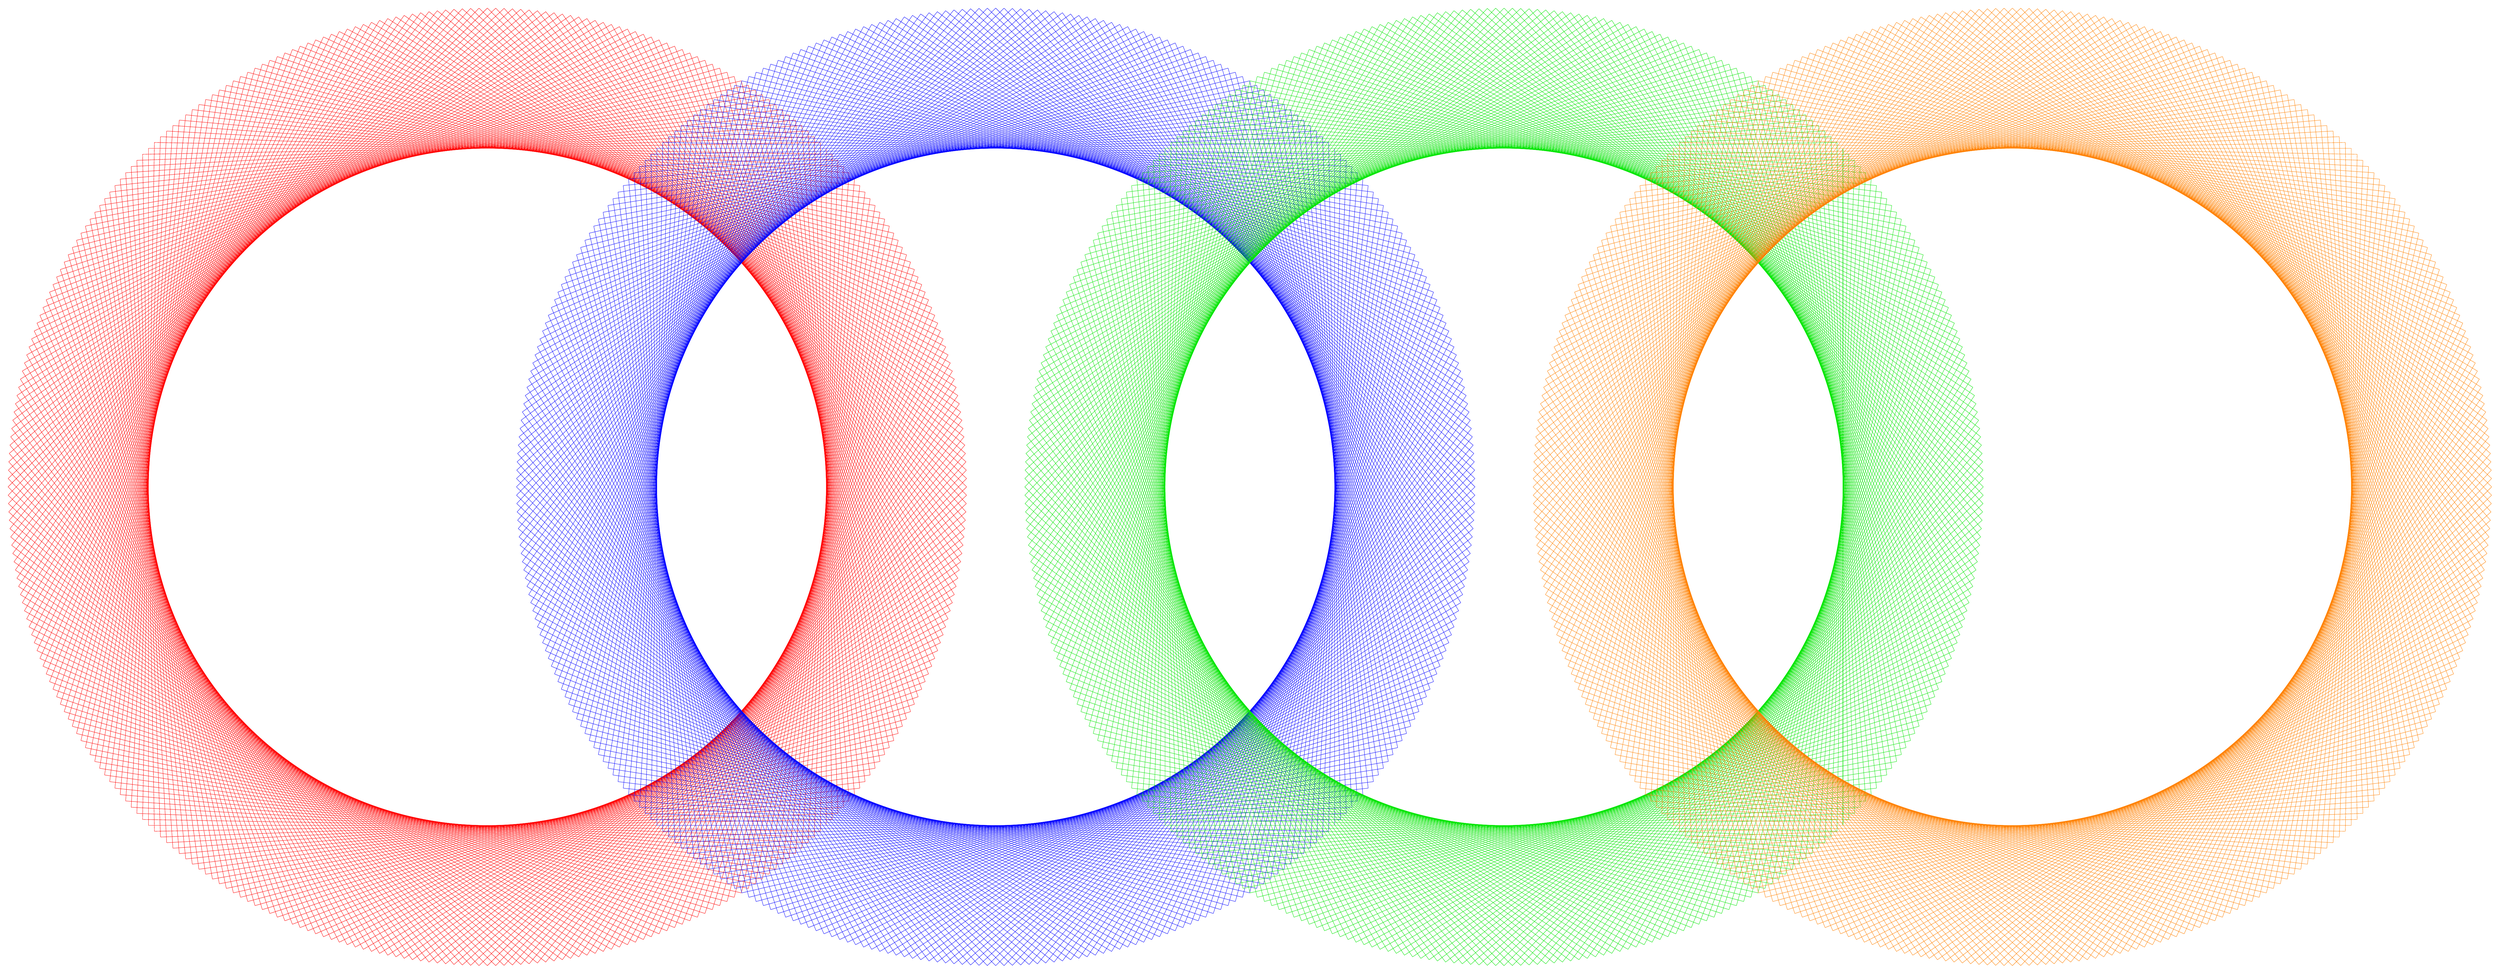
\begin{tikzpicture}[scale=3]

% 定义变量\step为1
\pgfmathsetmacro{\step}{1}
% 定义变量\max为\step变量-1
\pgfmathsetmacro{\max}{360-\step}

%\foreach \deg in {0,\step,...,\max} {
%    \draw [red, rotate around={\deg:(0,0)}] (-5,5) -- ++(10,0);
%}

\foreach \mcolor\rotcenter/\startx in {red/0/-5, blue/7.5/2.5, green!90!black/15/10, orange/22.5/17.5} {
    \foreach \deg in {0,\step,...,\max} {
        \draw [\mcolor, rotate around={\deg:(\rotcenter,0)}] (\startx,5) -- ++(10,0);
    }
}

\end{tikzpicture}
\end{document}
